\chapter{Méiose, brassage génétique et hérédité}\label{ch:b2:meiosis-heredity}

Deux parents aux yeux marron ont un enfant aux yeux bleus, et personne
ne s'en étonne~; deux enfants des mêmes parents ne se ressemblent jamais
tout à fait, et personne ne s'en étonne non plus. Les deux faits
découlent d'un même processus. À la formation de chaque ovocyte et de
chaque spermatozoïde, une cellule qui possède deux exemplaires de chaque
chromosome en transmet exactement un, choisi au hasard, après avoir
laissé les deux exemplaires échanger des segments. Chaque fécondation
réunit ensuite deux de ces demi-lots qui ne s'étaient jamais rencontrés.
Ce chapitre décrit ce processus --- la \omterm{def:b2:meiosis-heredity:meiosis}{méiose} --- et les règles de
l'hérédité qui en découlent~: les proportions de Mendel, leurs
exceptions, la liaison des gènes portés par un même chromosome et les
cartes qu'elle permet de tracer, et l'hérédité particulière des
\omterm{prop:b2:meiosis-heredity:sexlinked}{chromosomes sexuels} et des organites.

\section{La méiose}

\begin{definition}[Méiose]\label{def:b2:meiosis-heredity:meiosis}
\index{meiose@méiose}\index{haploide@haploïde}\index{diploide@diploïde}
Une cellule \emph{diploïde} ($2n$) porte deux chromosomes
\emph{homologues} de chaque type, un de chaque parent, semblables par
leur contenu en gènes mais pas nécessairement par leurs \omterm{def:b2:meiosis-heredity:vocabulary}{allèles}. La
\emph{méiose} est la succession de deux divisions qui transforme une
cellule diploïde en quatre cellules \emph{haploïdes} ($n$), chacune avec
un chromosome de chaque type. Elle est précédée d'une seule
réplication, si bien que chaque chromosome y entre sous la forme de
deux chromatides sœurs~; la première division sépare les
\emph{homologues} (division réductionnelle), la seconde sépare les
\emph{chromatides sœurs} (division équationnelle), comme le fait la
mitose. Chez les animaux, la méiose produit les gamètes~; chez les
plantes et les champignons, elle produit des spores
(\cref{ch:b2:plant-life-cycles})~; chez tout organisme sexué, c'est
l'étape qui divise par deux le nombre de chromosomes pour que la
fécondation puisse le doubler de nouveau.
\end{definition}

\begin{proposition}[Les étapes]\label{prop:b2:meiosis-heredity:stages}
\index{prophase I}\index{synapsis}\index{chiasma}\index{crossing-over}
La \emph{\omterm{prop:b2:meiosis-heredity:stages}{prophase I}} est longue, et c'est là que se fait le brassage.
Les chromosomes répliqués se condensent~; chacun trouve son homologue et
s'apparie avec lui gène à gène (\emph{synapsis}), maintenu par une
échelle protéique, le \emph{complexe synaptonémal}, pour former un
\emph{bivalent} de quatre chromatides~; des chromatides non sœurs se
cassent et se ressoudent en des points correspondants
(\emph{crossing-over}), une à plusieurs fois par bivalent~; lorsque le
complexe se dissout, les homologues ne restent attachés qu'en ces points
d'échange, visibles sous forme de \emph{chiasmas}.
\emph{Métaphase I}~: les bivalents s'alignent sur le fuseau, chaque
paire orientée au hasard --- l'homologue maternel vers un pôle ou vers
l'autre, indépendamment de toutes les autres paires. \emph{Anaphase I}~:
les homologues se séparent, les chromatides sœurs restant ensemble~;
chaque pôle reçoit $n$ chromosomes à deux chromatides. \emph{Télophase I}
puis, en général sans réplication, \emph{\omterm{def:b2:meiosis-heredity:meiosis}{méiose} II}~: les $n$
chromosomes s'alignent un par un, les chromatides sœurs se séparent, et
quatre noyaux \omterm{def:b2:meiosis-heredity:meiosis}{haploïdes} en résultent. La \omterm{def:b2:meiosis-heredity:meiosis}{méiose} I dure de quelques
heures à plusieurs décennies (un ovocyte humain reste en pause en
\omterm{prop:b2:meiosis-heredity:stages}{prophase I} depuis avant la naissance jusqu'à l'ovulation)~; la \omterm{def:b2:meiosis-heredity:meiosis}{méiose} II
dure une heure.
\end{proposition}

\begin{omfigure}
\begin{tikzpicture}[every node/.style={font=\scriptsize}]
  % helper: cell outline at (x,y)
  \foreach \x/\lab in {0/{prophase I~: appariement, crossing-over}, 3.2/{métaphase I~: bivalents alignés}, 6.4/{anaphase I~: les homologues se séparent}, 9.6/{méiose II~: les chromatides se séparent}}
    { \draw[thick] (\x+1.2,0) circle (1.15); \node[below, align=center, text width=2.8cm] at (\x+1.2,-1.2) {\lab}; }
  % prophase I: one bivalent with chiasma
  \draw[very thick, omDef] (0.8,-0.5) -- (0.8,0.5); \draw[very thick, omDef] (1.0,-0.5) -- (1.0,0.5);
  \draw[very thick, omThm] (1.4,-0.5) -- (1.4,0.5); \draw[very thick, omThm] (1.6,-0.5) -- (1.6,0.5);
  \draw[very thick, omDef] (1.0,0.1) -- (1.4,-0.1); \draw[very thick, omThm] (1.4,0.1) -- (1.0,-0.1);
  \fill[white] (0.9,-0.03) rectangle (1.5,0.03);
  \draw[very thick, omDef] (1.0,0.1) -- (1.4,-0.1); \draw[very thick, omThm] (1.4,0.1) -- (1.0,-0.1);
  \node[omExo!60!black] at (1.2,-0.85) {chiasma};
  % metaphase I: two bivalents on the plate, spindle
  \begin{scope}[xshift=3.2cm]
    \draw[gray, dashed] (1.2,-1.0) -- (1.2,1.0);
    \foreach \y in {0.45,-0.45} {
      \draw[very thick, omDef] (0.95,\y-0.25) -- (0.95,\y+0.25); \draw[very thick, omDef] (1.08,\y-0.25) -- (1.08,\y+0.25);
      \draw[very thick, omThm] (1.32,\y-0.25) -- (1.32,\y+0.25); \draw[very thick, omThm] (1.45,\y-0.25) -- (1.45,\y+0.25);
    }
    \draw[gray] (0.15,0) -- (0.95,0.45); \draw[gray] (0.15,0) -- (0.95,-0.45);
    \draw[gray] (2.25,0) -- (1.45,0.45); \draw[gray] (2.25,0) -- (1.45,-0.45);
  \end{scope}
  % anaphase I
  \begin{scope}[xshift=6.4cm]
    \foreach \y in {0.45,-0.45} {
      \draw[very thick, omDef] (0.45,\y-0.25) -- (0.45,\y+0.25); \draw[very thick, omDef] (0.58,\y-0.25) -- (0.58,\y+0.25);
      \draw[very thick, omThm] (1.82,\y-0.25) -- (1.82,\y+0.25); \draw[very thick, omThm] (1.95,\y-0.25) -- (1.95,\y+0.25);
    }
    \draw[->, gray] (1.2,0) -- (0.75,0); \draw[->, gray] (1.2,0) -- (1.65,0);
  \end{scope}
  % meiosis II: four cells
  \begin{scope}[xshift=9.6cm]
    \foreach \p/\c in {(0.75,0.5)/omDef,(1.65,0.5)/omDef,(0.75,-0.5)/omThm,(1.65,-0.5)/omThm} {
      \draw[thick, gray!60] \p circle (0.38);
      \draw[very thick, \c] \p ++(-0.12,-0.2) -- ++(0,0.4);
      \draw[very thick, \c] \p ++(0.12,-0.2) -- ++(0,0.4);
    }
  \end{scope}
\end{tikzpicture}

{\small La \omterm{def:b2:meiosis-heredity:meiosis}{méiose} pour deux paires d'homologues (maternels en bleu,
paternels en rouge, chacun à deux chromatides). Les homologues
s'apparient et échangent des segments en \omterm{prop:b2:meiosis-heredity:stages}{prophase I}, s'alignent en
bivalents en métaphase I, se séparent en anaphase I~; la \omterm{def:b2:meiosis-heredity:meiosis}{méiose} II
sépare les chromatides en quatre cellules \omterm{def:b2:meiosis-heredity:meiosis}{haploïdes}.}
\end{omfigure}

\begin{omfigure}
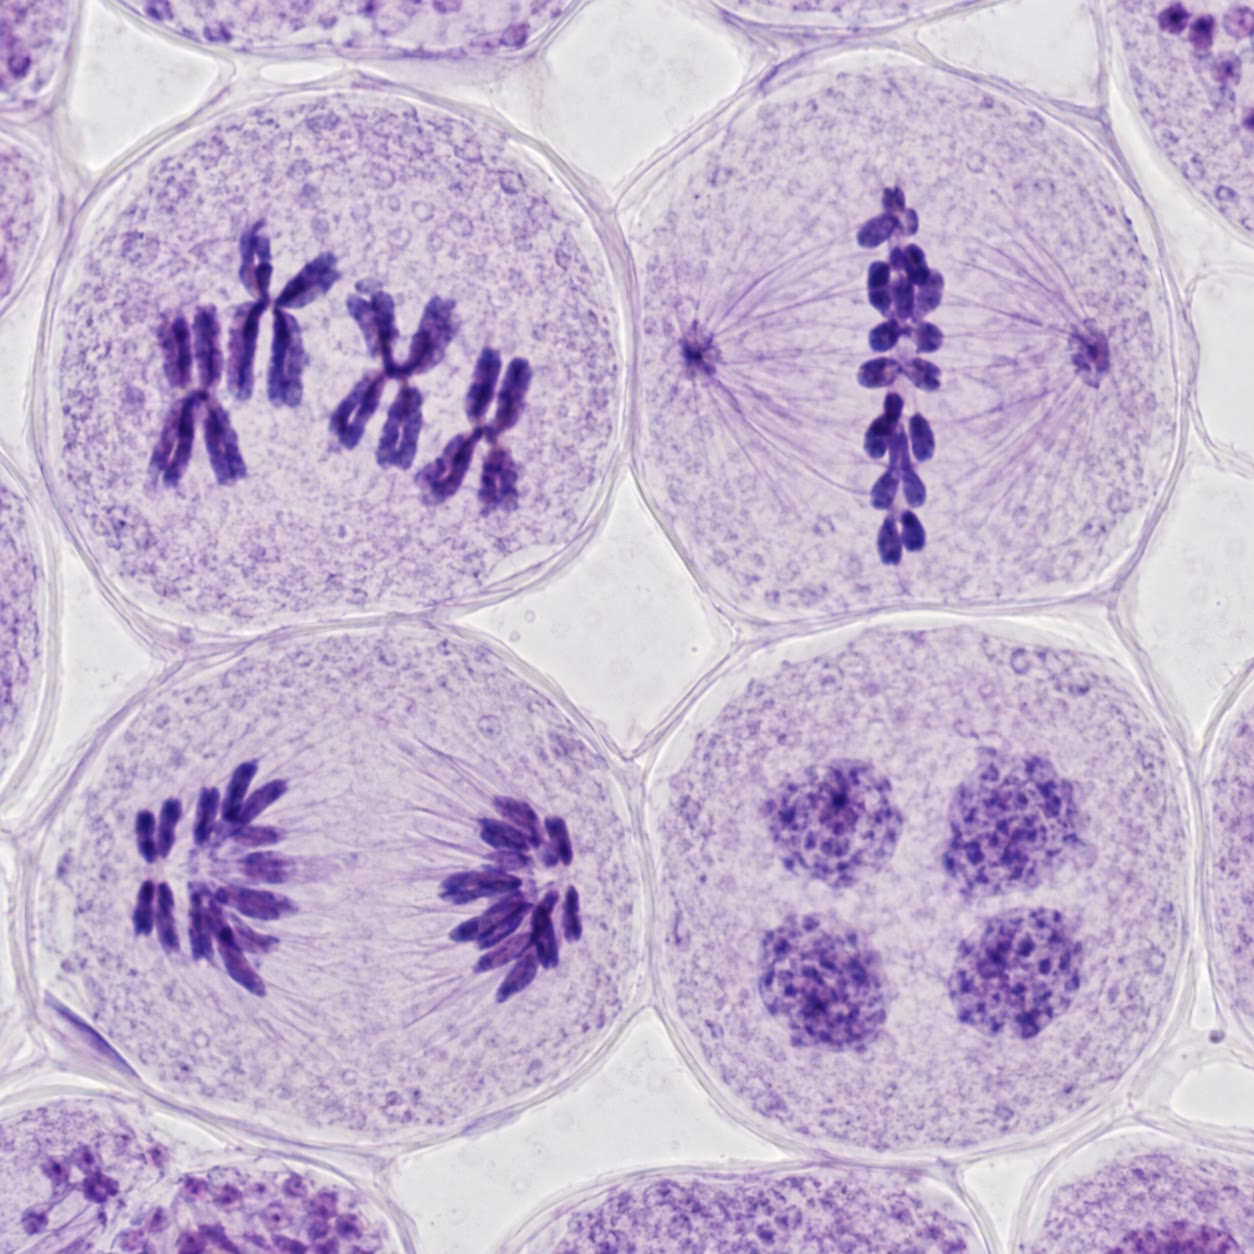
\includegraphics[width=0.5\linewidth]{images/book4/ai/b4-04-lily-meiosis.jpg}

{\small La \omterm{def:b2:meiosis-heredity:meiosis}{méiose} dans l'anthère d'un lis~: des bivalents en fin de
\omterm{prop:b2:meiosis-heredity:stages}{prophase I}, une plaque métaphasique I, une anaphase I, et les quatre
noyaux d'une tétrade.}
\end{omfigure}

\begin{theorem}[Quel brassage produit la méiose]\label{thm:b2:meiosis-heredity:mixing}
\index{brassage interchromosomique}\index{recombinaison genetique@recombinaison génétique}
Pour un organisme à $n$ paires de chromosomes, l'orientation aléatoire
des bivalents en métaphase I produit $2^n$ combinaisons possibles de
chromosomes maternels et paternels dans un gamète ---
$2^{23} \approx 8.4$ millions chez l'être humain --- et $2^{2n}$ dans
un zygote. Le crossing-over multiplie ce nombre~: avec environ $k$
chiasmas par bivalent, chacun en une position variable, le nombre de
gamètes distincts est en pratique illimité, et deux gamètes d'une même
personne ne sont jamais identiques. La \emph{recombinaison} --- de
nouvelles combinaisons d'\omterm{def:b2:meiosis-heredity:vocabulary}{allèles} --- naît des deux processus~: le
\omterm{thm:b2:meiosis-heredity:mixing}{brassage interchromosomique} rebat des chromosomes entiers, le
crossing-over rebat des gènes au sein d'un chromosome.
\end{theorem}
\begin{proof}
Chaque bivalent s'oriente indépendamment selon deux issues~: $n$
bivalents donnent donc $2^n$ combinaisons, toutes équiprobables. Chacun
des deux parents fournit un tel gamète, si bien que le zygote en compte
$2^n\times
2^n$. Un crossing-over en une position distincte d'un chromosome de $L$
paires de bases peut produire de l'ordre de $L$ chromatides
recombinées distinctes par bivalent~; le nombre de produits distincts
croît donc comme $L^k$ par chromosome, ce qui est astronomique pour
$L \sim 10^8$.
\end{proof}
\begin{proof}[Faits expérimentaux]
Creighton et McClintock (1931) utilisèrent un chromosome 9 de maïs qui
portait deux marques cytologiques visibles (un bouton à une extrémité,
un segment transloqué à l'autre) et deux gènes entre elles (grain coloré
ou incolore, albumen cireux ou amylacé). Dans la descendance, toute
plante porteuse d'une paire d'\omterm{def:b2:meiosis-heredity:vocabulary}{allèles} recombinée portait aussi une
paire recombinée de marques cytologiques --- bouton sans translocation
ou l'inverse --- ce qui prouvait que la \omterm{thm:b2:meiosis-heredity:mixing}{recombinaison génétique} est un
échange physique de segments de chromosomes.
\end{proof}

\begin{omfigure}
\begin{tikzpicture}[every node/.style={font=\scriptsize}]
  \foreach \dx/\lab/\ca/\cb/\gam in {0/{orientation 1}/omDef/omThm/{gamètes AB et ab}, 6.2/{orientation 2}/omThm/omDef/{gamètes Ab et aB}} {
    \begin{scope}[xshift=\dx cm]
      \draw[gray, dashed] (0,-1.1) -- (3.2,-1.1);
      \node[anchor=south] at (1.6,0.6) {\lab};
      % pair 1 (long): A above the plate, a below
      \draw[very thick, omDef] (0.7,-0.95) -- (0.7,-0.25); \node[omDef, anchor=south] at (0.7,-0.2) {A};
      \draw[very thick, omThm] (0.7,-1.25) -- (0.7,-1.95); \node[omThm, anchor=north] at (0.7,-2.0) {a};
      % pair 2 (short): B or b above depending on orientation
      \draw[very thick, \ca] (2.3,-0.85) -- (2.3,-0.35);
      \draw[very thick, \cb] (2.3,-1.35) -- (2.3,-1.85);
      \node[anchor=north] at (1.6,-2.4) {\gam};
    \end{scope}
  }
  \node[omDef, anchor=south] at (2.3,-0.3) {B}; \node[omThm, anchor=north] at (2.3,-1.9) {b};
  \node[omThm, anchor=south] at (8.5,-0.3) {b}; \node[omDef, anchor=north] at (8.5,-1.9) {B};
  \node[anchor=north, align=center] at (4.7,-3.0) {chaque orientation est équiprobable~:\\gamètes AB, ab, Ab, aB en nombres égaux --- brassage interchromosomique};
\end{tikzpicture}

{\small Le \omterm{thm:b2:meiosis-heredity:mixing}{brassage interchromosomique}. Pour deux paires de chromosomes
(A/a sur l'une, B/b sur l'autre), les deux orientations possibles des
bivalents en métaphase I sont équiprobables~; les quatre combinaisons
d'\omterm{def:b2:meiosis-heredity:vocabulary}{allèles} apparaissent donc en nombres égaux parmi les gamètes.}
\end{omfigure}

\section{L'analyse mendélienne}

\begin{definition}[Le vocabulaire des croisements]\label{def:b2:meiosis-heredity:vocabulary}
\index{allele@allèle}\index{genotype@génotype}\index{phenotype@phénotype}\index{dominant}\index{recessif@récessif}\index{homozygote}\index{heterozygote@hétérozygote}
Un \emph{gène} est un segment de chromosome~; ses \emph{allèles} sont
ses variants de séquence~; le \emph{locus} est sa position. Un individu
\omterm{def:b2:meiosis-heredity:meiosis}{diploïde} porte deux allèles à chaque locus~: son \emph{génotype}
est \emph{homozygote} ($AA$, $aa$) ou \emph{hétérozygote} ($Aa$).
Le \emph{phénotype} est le caractère observable. Un allèle est
\emph{dominant} lorsque l'hétérozygote présente son phénotype,
\emph{récessif} lorsqu'il ne s'exprime que chez l'homozygote~; cette
distinction est une propriété de la paire d'allèles et du caractère
observé, non de l'allèle seul --- la plupart des allèles récessifs sont
des allèles perte de fonction, masqués parce qu'une seule copie
fonctionnelle suffit. Une \emph{lignée pure} se reproduit à l'identique
(homozygote)~; un \emph{croisement-test} croise un individu de phénotype
dominant avec un homozygote récessif, de sorte que sa descendance révèle
directement les allèles de ses gamètes.
\end{definition}

\begin{theorem}[Les proportions de Mendel]\label{thm:b2:meiosis-heredity:mendel}
\index{lois de Mendel}\index{croisement monohybride}\index{croisement dihybride}
Comme les deux \omterm{def:b2:meiosis-heredity:vocabulary}{allèles} d'un \omterm{def:b2:meiosis-heredity:vocabulary}{hétérozygote} $Aa$ ségrègent dans des
gamètes différents en nombres égaux (anaphase I), un croisement
\emph{monohybride} $Aa \times Aa$ donne les \omterm{def:b2:meiosis-heredity:vocabulary}{génotypes} $\tfrac14 AA : \tfrac12 Aa :
\tfrac14 aa$, et les \omterm{def:b2:meiosis-heredity:vocabulary}{phénotypes} $3 : 1$ si $A$ est \omterm{def:b2:meiosis-heredity:vocabulary}{dominant}~; le
croisement-test
$Aa \times aa$ donne $1 : 1$. Comme les \omterm{def:b2:meiosis-heredity:vocabulary}{allèles} de gènes situés sur des
chromosomes différents ségrègent indépendamment (métaphase I), un
\emph{dihybride}
$AaBb$ produit quatre types de gamètes en nombres égaux, et le croisement
$AaBb \times AaBb$ donne les \omterm{def:b2:meiosis-heredity:vocabulary}{phénotypes} $9 : 3 : 3 : 1$, le
croisement-test
$AaBb \times aabb$ donnant $1 : 1 : 1 : 1$. Pour $k$ loci \omterm{def:b2:meiosis-heredity:vocabulary}{hétérozygotes}
indépendants, le nombre de types de gamètes est $2^k$ et la proportion
phénotypique est le produit de $k$ proportions $3 : 1$.
\end{theorem}
\begin{proof}
Ségrégation~: les gamètes de l'\omterm{def:b2:meiosis-heredity:vocabulary}{hétérozygote} sont $\tfrac12 A$,
$\tfrac12 a$~; avec une fécondation au hasard, les \omterm{def:b2:meiosis-heredity:vocabulary}{génotypes} des
zygotes sont les produits $(\tfrac12 A + \tfrac12 a)^2 = \tfrac14 AA + \tfrac12 Aa +
\tfrac14 aa$. Indépendance~: les gamètes de $AaBb$ sont $(\tfrac12 A
+ \tfrac12 a)(\tfrac12 B + \tfrac12 b)$, quatre types à $\tfrac14$~;
les \omterm{def:b2:meiosis-heredity:vocabulary}{phénotypes} du dihybride se multiplient $(\tfrac34 A\_ + \tfrac14 aa)
(\tfrac34 B\_ + \tfrac14 bb)$, ce qui donne $\tfrac{9}{16}, \tfrac{3}{16},
\tfrac{3}{16}, \tfrac{1}{16}$. Chaque facteur est une ségrégation
indépendante~: $k$ loci donnent donc un produit de $k$ facteurs.
\end{proof}
\begin{proof}[Faits expérimentaux]
Mendel (1866) croisa des lignées pures de pois différant par un
caractère --- graine lisse ou ridée, cotylédon jaune ou vert, fleur
pourpre ou blanche, tige haute ou naine, et trois autres --- et trouva
dans tous les cas une première génération uniforme et une deuxième
génération ségrégeant près de $3 : 1$~: 5474 lisses pour 1850 ridées
($2.96 :
1$), 6022 jaunes pour 2001 vertes ($3.01 : 1$), 705 pourpres pour 224
blanches
($3.15 : 1$). Dans les croisements à deux caractères, il trouva $315 : 108 : 101 :
32$ ($9 : 3 : 3 : 1$), et en cultivant la deuxième génération, il
montra que la classe dominante était de deux sortes, un tiers pur et
deux tiers en ségrégation. Les chromosomes qui expliquent ces
proportions furent découverts quarante ans plus tard.
\end{proof}

\begin{omfigure}
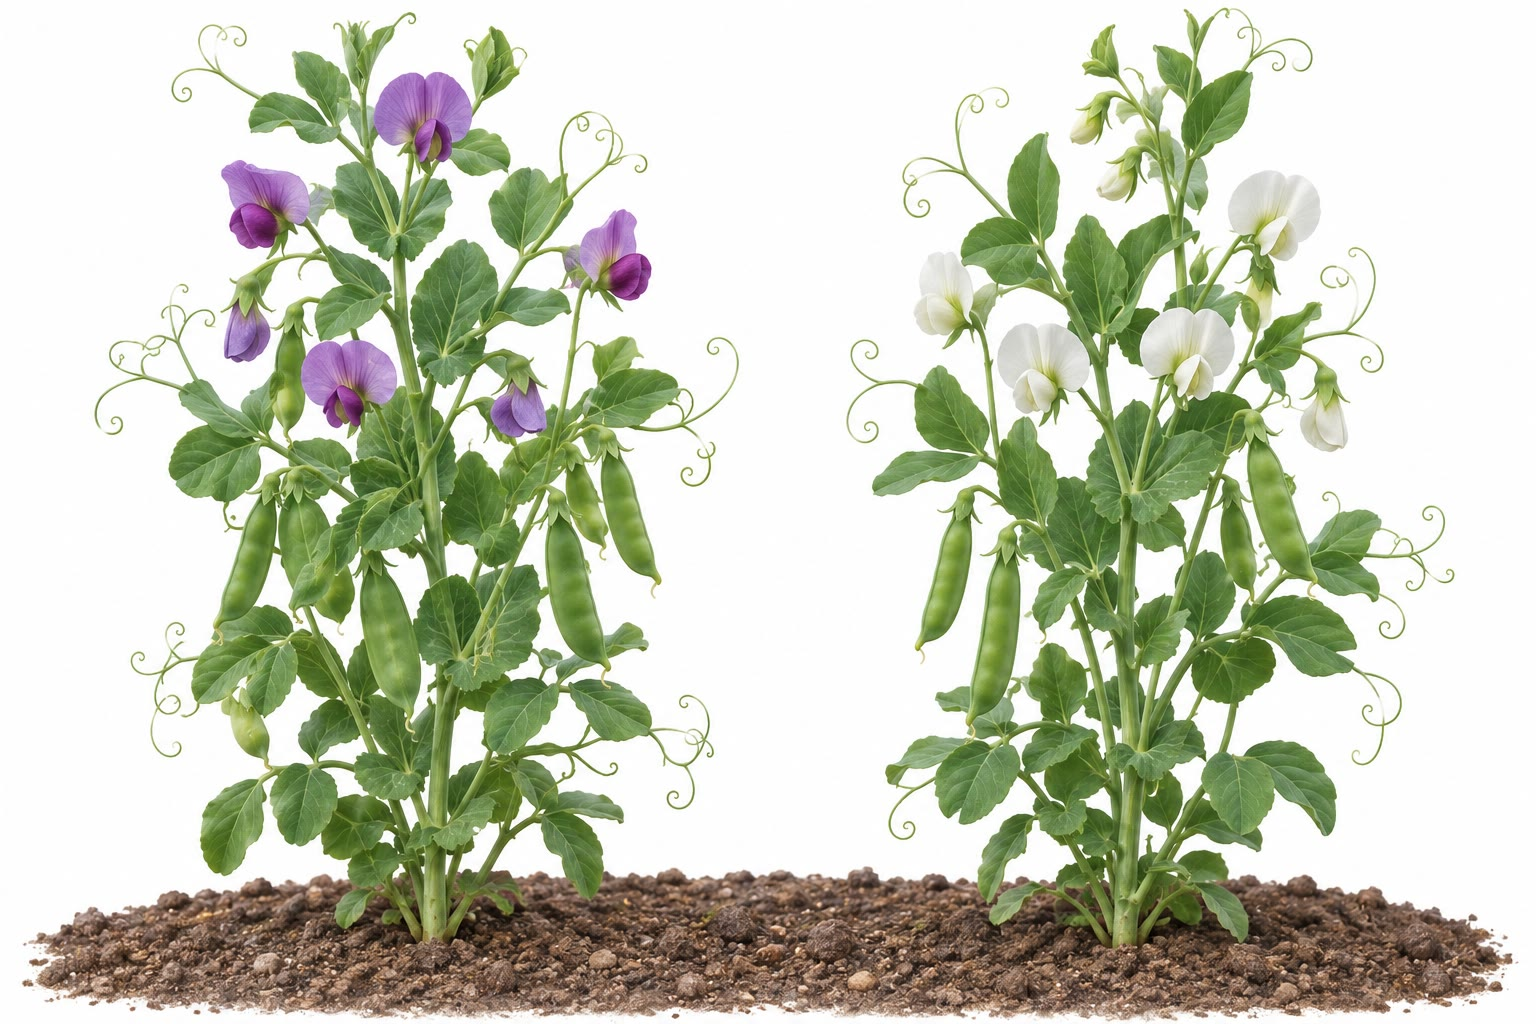
\includegraphics[width=0.58\linewidth]{images/book4/ai/b4-04-pea-flowers.jpg}

{\small Plants de pois à fleurs pourpres et à fleurs blanches~: l'une
des sept paires de caractères sur lesquelles Mendel fonda la génétique.
L'hybride à fleurs pourpres, autofécondé, donne environ trois pourpres
pour une blanche.}
\end{omfigure}

\begin{method}[Tester une proportion avec le $\chi^2$]\label{met:b2:meiosis-heredity:chisquare}
\index{test du chi-deux}
Pour décider si des effectifs observés $O_i$ s'accordent avec une
proportion supposée~:
\begin{enumerate}
  \item Calculer les effectifs attendus $E_i$ à partir de la proportion
        et du total.
  \item Calculer $\chi^2 = \sum_i (O_i - E_i)^2/E_i$.
  \item Compter les degrés de liberté~: le nombre de classes moins un.
  \item Comparer à la valeur critique au seuil de \qty{5}{\%}~:
        $3.84$ pour 1 degré de liberté, $5.99$ pour 2, $7.81$ pour 3,
        $9.49$ pour 4. Si $\chi^2$ lui est inférieur, les données sont
        compatibles avec la proportion~; s'il est supérieur, la
        proportion est rejetée --- l'écart ne se produirait par hasard
        que dans moins d'une expérience sur vingt.
\end{enumerate}
Pour les fleurs de Mendel, $705 : 224$ contre $3 : 1$~: $E = 696.75,
232.25$~; $\chi^2 = 0.098 + 0.293 = 0.39 < 3.84$. (La loi qui sous-tend
les valeurs critiques est établie dans la partie statistique de la
série de mathématiques~; ici, la table est un outil.)
\end{method}

\begin{proposition}[Au-delà des proportions simples]\label{prop:b2:meiosis-heredity:extensions}
\index{dominance incomplete@dominance incomplète}\index{codominance}\index{epistasie@épistasie}\index{allele letal@allèle létal}
Les proportions changent, mais non le mécanisme, lorsque~: les \omterm{def:b2:meiosis-heredity:vocabulary}{allèles}
présentent une \emph{\omterm{prop:b2:meiosis-heredity:extensions}{dominance incomplète}} (un muflier rouge $\times$
blanc donne des fleurs roses, et la deuxième génération $1 : 2 : 1$)~;
les \omterm{def:b2:meiosis-heredity:vocabulary}{allèles} sont \emph{codominants}, tous deux exprimés (groupe
sanguin $AB$~: l'\omterm{def:b2:meiosis-heredity:vocabulary}{hétérozygote} $I^AI^B$ fabrique les deux antigènes~; un locus
peut avoir des \emph{\omterm{def:b2:meiosis-heredity:vocabulary}{allèles} multiples}, $I^A$, $I^B$, $i$)~; un \omterm{def:b2:meiosis-heredity:vocabulary}{allèle}
est \emph{létal} à l'état \omterm{def:b2:meiosis-heredity:vocabulary}{homozygote} (souris jaunes~: jaune $\times$
jaune donne $2$ jaunes pour
$1$ agouti, les $\tfrac14 YY$ mourant à l'état d'embryons)~; deux gènes
agissent dans une même voie (\emph{épistasie}~: dans un croisement
$9 : 3 : 3 : 1$, le double \omterm{def:b2:meiosis-heredity:vocabulary}{récessif} et un simple \omterm{def:b2:meiosis-heredity:vocabulary}{récessif} peuvent être
indiscernables, ce qui donne
$9 : 3 : 4$, comme pour les souris albinos, ou les deux \omterm{def:b2:meiosis-heredity:vocabulary}{dominants}
peuvent être tous deux nécessaires au \omterm{def:b2:meiosis-heredity:vocabulary}{phénotype}, ce qui donne $9 : 7$,
comme pour les pois de senteur pourpres, qui ont besoin de deux enzymes
pour fabriquer leur pigment)~; de nombreux gènes ajoutent chacun un peu
à un caractère continu (taille, rendement), ce qui relève de la
génétique quantitative du \cref{ch:b2:population-genetics}. Remonter
d'une proportion à un mécanisme est le savoir-faire quotidien de la
génétique.
\end{proposition}

\section{Liaison génétique et cartes génétiques}

\begin{definition}[Liaison et fréquence de recombinaison]\label{def:b2:meiosis-heredity:linkage}
\index{liaison genetique@liaison génétique}\index{frequence de recombinaison@fréquence de recombinaison}\index{centimorgan}
Deux gènes portés par un même chromosome sont \emph{liés}~: leurs
\omterm{def:b2:meiosis-heredity:vocabulary}{allèles} tendent à passer ensemble dans les gamètes, et un dihybride
$AB/ab$ produit plus de gamètes \emph{parentaux} ($AB$, $ab$) que de
gamètes \emph{recombinés} ($Ab$, $aB$). Les recombinés n'apparaissent
que si un crossing-over se produit entre les deux loci~; leur fréquence
$r$ --- comptée directement dans un croisement-test --- mesure donc la
distance~: $r$ va de 0 (liaison complète) à $\tfrac12$ (gènes si
éloignés, ou situés sur des chromosomes différents, qu'ils ségrègent
indépendamment). L'unité de \emph{distance génétique} est le
\emph{centimorgan} (cM)~: \qty{1}{cM}
correspond à \qty{1}{\%} de recombinaison pour des gènes étroitement
liés~; chez l'être humain, \qty{1}{cM} vaut environ un million de paires
de bases. La liaison fut la première preuve que les gènes sont alignés
sur le chromosome.
\end{definition}
\begin{proof}[Faits expérimentaux]
Morgan (1911) constata que les gènes «~yeux blancs~» et «~ailes
miniatures~» de la drosophile, tous deux portés
par le chromosome X, ne ségrégeaient pas indépendamment~: un
croisement-test donnait \qty{37}{\%} de recombinés au lieu de
\qty{50}{\%}, et d'autres paires donnaient d'autres pourcentages,
reproductibles. Sturtevant (1913), alors étudiant, comprit que si ces
fréquences mesurent des distances, elles doivent s'additionner~: à
partir des fréquences deux à deux de six gènes liés à l'X, il traça la
première carte génétique, et les distances étaient, aux erreurs près,
additives le long d'une ligne.
\end{proof}

\begin{omfigure}
\begin{tikzpicture}[every node/.style={font=\scriptsize}]
  % bivalent with crossover between A and B
  \draw[very thick, omDef] (0,1.2) -- (2.0,1.2) -- (3.0,0.6) -- (5,0.6);
  \draw[very thick, omDef] (0,1.5) -- (5,1.5);
  \draw[very thick, omThm] (0,0.3) -- (2.0,0.3) -- (3.0,0.9) -- (5,0.9);
  \draw[very thick, omThm] (0,0) -- (5,0);
  \node[omDef, above] at (0.8,1.5) {A}; \node[omDef, above] at (4.3,1.5) {B};
  \node[omThm, below] at (0.8,0) {a}; \node[omThm, below] at (4.3,0) {b};
  \node[anchor=south, gray] at (2.5,1.85) {crossing-over entre les loci A et B};
  % products
  \draw[->, thick, gray] (5.4,0.75) -- (6.2,0.75);
  \node[anchor=west, align=left] at (6.4,1.45) {\textcolor{omDef}{A\,B} \quad parental};
  \node[anchor=west, align=left] at (6.4,0.95) {\textcolor{omDef}{A}\,\textcolor{omThm}{b} \quad recombiné};
  \node[anchor=west, align=left] at (6.4,0.5) {\textcolor{omThm}{a}\,\textcolor{omDef}{B} \quad recombiné};
  \node[anchor=west, align=left] at (6.4,0.0) {\textcolor{omThm}{a\,b} \quad parental};
  \node[anchor=west, align=left, text width=5.6cm] at (6.4,-0.9) {un crossing-over entre les loci dans une fraction $c$ des méioses~: gamètes recombinés $r = c/2$, car seules deux des quatre chromatides sont échangées};
\end{tikzpicture}

{\small La recombinaison entre deux loci liés. Un crossing-over entre
eux dans un bivalent échange les \omterm{def:b2:meiosis-heredity:vocabulary}{allèles} de deux des quatre
chromatides~; les gamètes recombinés sont comptés dans un
croisement-test, et leur fréquence mesure la distance.}
\end{omfigure}

\begin{method}[Cartographier deux gènes liés]\label{met:b2:meiosis-heredity:twopoint}
\begin{enumerate}
  \item Croiser deux lignées pures pour obtenir le dihybride~; noter
        quels \omterm{def:b2:meiosis-heredity:vocabulary}{allèles} il a reçus ensemble (ses combinaisons parentales,
        en \emph{couplage} $AB/ab$ ou en \emph{répulsion} $Ab/aB$).
  \item Le croiser avec le double \omterm{def:b2:meiosis-heredity:vocabulary}{récessif} et classer la descendance~:
        les deux classes les plus nombreuses sont parentales, les deux
        moins nombreuses recombinées.
  \item $r = $ recombinés $/$ total~; la distance vaut $100\,r$ cM.
  \item Vérifier d'abord l'indépendance~: si les quatre classes sont
        égales ($\chi^2$ contre $1 : 1 : 1 : 1$), les gènes ne sont pas
        liés.
\end{enumerate}
\end{method}

\begin{theorem}[La fonction de cartographie de Haldane]\label{thm:b2:meiosis-heredity:haldane}
\index{fonction de cartographie}
La \omterm{def:b2:meiosis-heredity:linkage}{fréquence de recombinaison} sous-estime la distance entre gènes
éloignés, car deux crossing-over entre eux restaurent la combinaison
parentale. Si les crossing-over se répartissent indépendamment le long
du chromosome (sans interférence), $d$ étant la distance génétique en
morgans (nombre attendu de crossing-over par chromatide), la fraction
de recombinaison vaut
\[
r = \tfrac12\,\bigl(1 - e^{-2d}\bigr), \qquad d = -\tfrac12\ln(1 - 2r),
\]
de sorte que $r \approx d$ pour $d$ petit et $r \to \tfrac12$ quand $d$
croît~; $r = 0.40$ correspond à \qty{80}{cM}, et \qty{50}{cM}
donne $r = 0.32$. Les chromosomes réels présentent une
\emph{interférence} --- un crossing-over rend moins probable un autre
crossing-over à proximité --- qui rapproche $r$ de $d$ davantage que ne
le prévoit Haldane sur de courtes distances.
\end{theorem}
\begin{proof}
Soit $d$ la distance génétique, nombre attendu de crossing-over par
chromatide dans l'intervalle~; comme chaque crossing-over implique deux
des quatre chromatides, le bivalent entier porte dans l'intervalle un
nombre de crossing-over distribué selon une loi de Poisson de moyenne
$2d$, et la probabilité qu'il n'en porte aucun vaut $e^{-2d}$. S'il en
porte au moins un, chaque crossing-over implique indépendamment une
chromatide donnée avec une probabilité
$\tfrac12$~: une chromatide donnée a donc été échangée un nombre impair
de fois --- elle est recombinée --- avec une probabilité exactement
égale à $\tfrac12$, quel que soit le nombre de crossing-over. D'où $r = \tfrac12\,(1 -
e^{-2d})$~; en inversant, on obtient $d$. Pour $d$ petit, $r \approx d$~;
quand $d \to \infty$, $r \to \tfrac12$.
\end{proof}

\begin{omfigure}
\begin{tikzpicture}
\begin{axis}[
  width=0.72\linewidth, height=5.6cm,
  axis x line=bottom, axis y line=left,
  xmin=0, xmax=150, ymin=0, ymax=0.55,
  xlabel={distance génétique $d$ (cM)}, ylabel={fraction de recombinaison $r$},
  xlabel style={font=\small, at={(axis description cs:0.5,-0.13)}, anchor=north},
  ylabel style={font=\small},
  tick label style={font=\small}, xtick={0,50,100,150}, ytick={0,0.25,0.5},
  legend style={font=\scriptsize, at={(0.97,0.1)}, anchor=south east, draw=none},
  clip=false,
]
\addplot[very thick, omDef, domain=0:150, samples=80] {0.5*(1-exp(-2*x/100))};
\addlegendentry{Haldane~: $r = \tfrac12(1 - e^{-2d})$}
\addplot[thick, dashed, gray, domain=0:50, samples=2] {x/100};
\addlegendentry{$r = d$ (sans double crossing-over)}
\draw[dashed, gray] (axis cs:0,0.5) -- (axis cs:150,0.5);
\end{axis}
\end{tikzpicture}

{\small Fraction de recombinaison en fonction de la distance génétique.
Des gènes proches recombinent en proportion de leur distance~; des gènes
éloignés ne dépassent jamais \qty{50}{\%} de recombinaison, quelle que
soit leur distance, car les doubles crossing-over restaurent les
combinaisons parentales.}
\end{omfigure}

\begin{method}[Le croisement-test à trois points]\label{met:b2:meiosis-heredity:threepoint}
\index{croisement a trois points@croisement à trois points}\index{interference@interférence}
Croiser un triple \omterm{def:b2:meiosis-heredity:vocabulary}{hétérozygote} $ABC/abc$ avec $abc/abc$ et classer les
huit classes de descendants.
\begin{enumerate}
  \item Les deux classes les plus nombreuses sont les parentales~; les
        deux moins nombreuses sont les \emph{doubles crossing-over}.
  \item Le gène qui change entre une classe parentale et la classe
        double crossing-over est celui du \emph{milieu}~: cela donne
        l'ordre.
  \item Pour chaque paire de gènes adjacents, la \omterm{def:b2:meiosis-heredity:linkage}{fréquence de
        recombinaison} vaut (simples crossing-over dans cet intervalle
        + doubles crossing-over) $/$ total, car un double crossing-over
        recombine les deux intervalles.
  \item Doubles crossing-over attendus $= r_1 r_2 \times$ total~; le
        \emph{coefficient de coïncidence} est le rapport observé/attendu
        et l'\emph{interférence} vaut $1 -$ coïncidence.
\end{enumerate}
\end{method}

\begin{example}[Un croisement à trois points résolu]\label{ex:b2:meiosis-heredity:threepoint}
Descendance de $+++/abc \times abc/abc$~: $+++$ 580, $abc$ 592, $++c$
45, $ab+$ 40, $+bc$ 89, $a++$ 94, $+b+$ 3, $a+c$ 5~; total 1448.
Parentaux $+++$, $abc$~; doubles $+b+$, $a+c$~; en comparant $+++$ à
$+b+$, le gène qui a changé est $b$~: ordre $a$--$b$--$c$. $r_{ab} =
(89 + 94 + 3 + 5)/1448 = 0.132$~; $r_{bc} = (45 + 40 + 3 + 5)/1448 =
0.064$~; carte~: $a$ --- \qty{13.2}{cM} --- $b$ --- \qty{6.4}{cM} ---
$c$. Doubles attendus $0.132\times 0.064\times 1448 = 12.2$,
observés 8~: coïncidence $0.65$, interférence $0.35$.
\end{example}

\begin{omfigure}
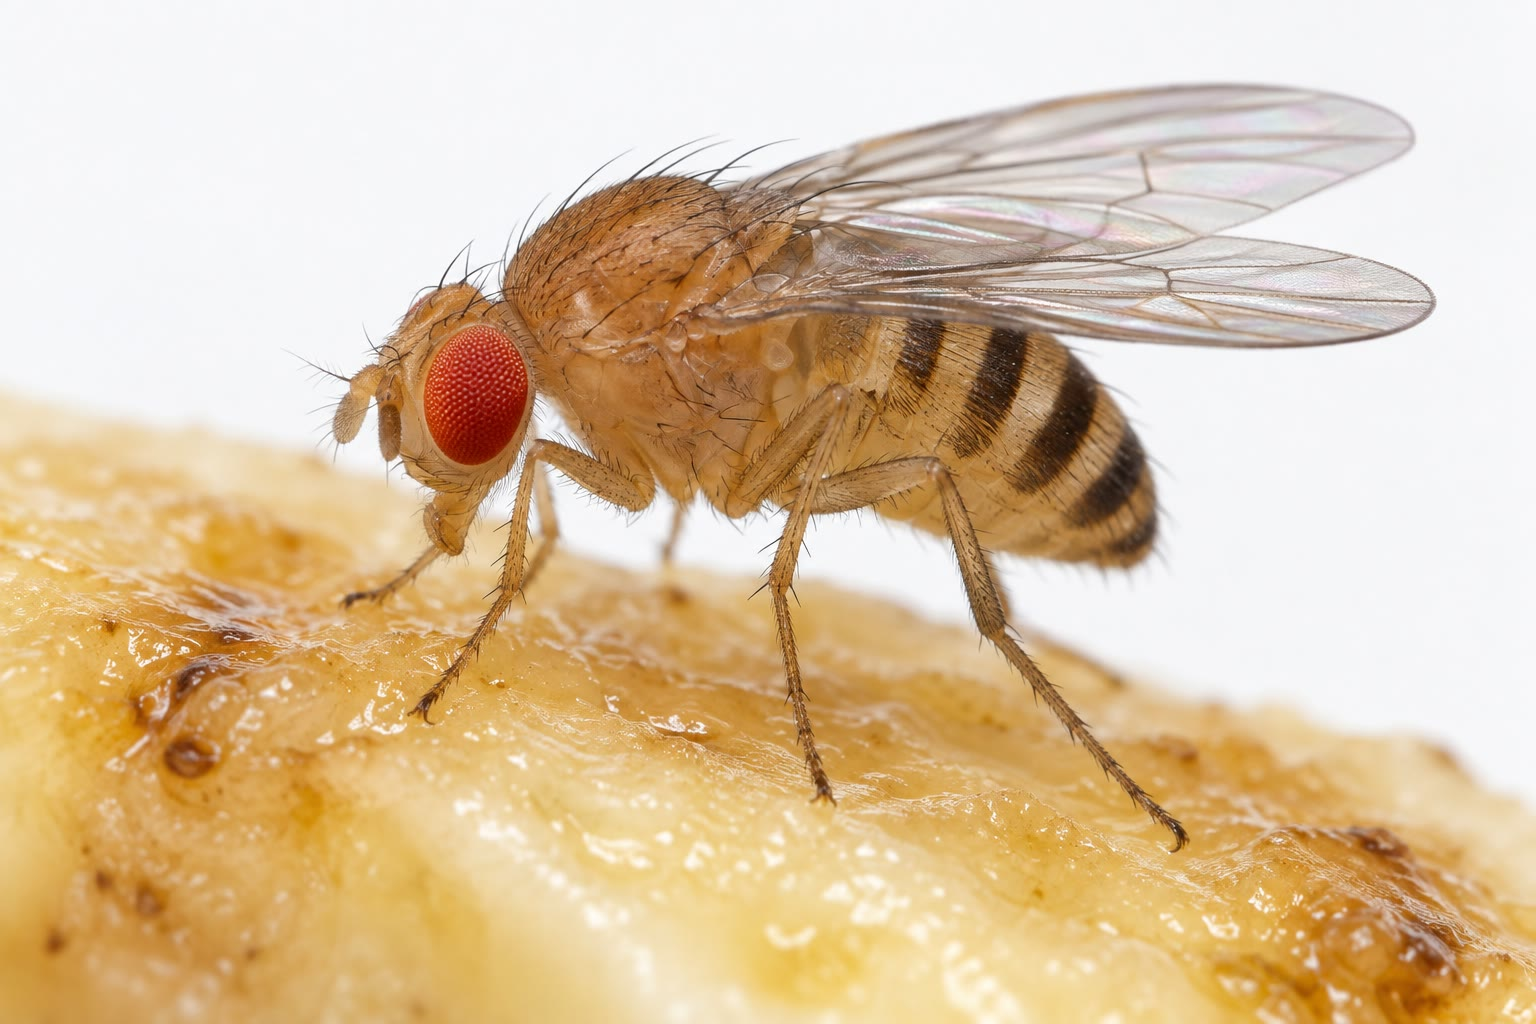
\includegraphics[width=0.5\linewidth]{images/book4/ai/b4-04-drosophila.jpg}

{\small \emph{Drosophila melanogaster}~: deux semaines par génération,
des centaines de descendants, quatre paires de chromosomes et un siècle
de mutants --- l'organisme sur lequel furent établies la liaison, les
cartes et l'hérédité liée au sexe.}
\end{omfigure}

\section{Chromosomes sexuels et organites}

\begin{proposition}[L'hérédité liée au sexe]\label{prop:b2:meiosis-heredity:sexlinked}
\index{heredite liee a l'X@hérédité liée à l'X}\index{chromosomes sexuels}
Chez les mammifères et les mouches, la femelle est $XX$ et le mâle
$XY$~: le $Y$ porte peu de gènes, si bien qu'un mâle possède un seul
exemplaire de chaque gène lié à l'$X$ (il est \emph{hémizygote}) et
exprime l'\omterm{def:b2:meiosis-heredity:vocabulary}{allèle} qu'il porte, qu'il soit \omterm{def:b2:meiosis-heredity:vocabulary}{dominant} ou \omterm{def:b2:meiosis-heredity:vocabulary}{récessif}.
Conséquences~: les croisements réciproques diffèrent (femelle aux yeux
blancs $\times$ mâle aux yeux rouges donne des fils aux yeux blancs et
des filles aux yeux rouges~; le croisement inverse donne une
descendance toute rouge)~; un caractère \omterm{def:b2:meiosis-heredity:vocabulary}{récessif} lié à l'$X$
(daltonisme rouge--vert, hémophilie, myopathie de Duchenne) apparaît
surtout chez les garçons, est transmis par des mères conductrices non
atteintes, et n'est jamais transmis de père à fils (un fils reçoit le
$Y$ de son père)~; un père transmet son $X$ à toutes ses filles. Les
oiseaux, les papillons et certains reptiles inversent le dispositif
(femelles $ZW$, mâles $ZZ$)~; chez de nombreux reptiles, c'est la
température qui décide~; et chez les mammifères, un $X$ de chaque
cellule femelle est inactivé au hasard tôt au cours du développement,
si bien qu'une femelle \omterm{def:b2:meiosis-heredity:vocabulary}{hétérozygote} est une mosaïque (la chatte
écaille de tortue).
\end{proposition}
\begin{proof}[Faits expérimentaux]
Morgan (1910) trouva un mâle aux yeux blancs parmi des milliers de
mouches aux yeux rouges. Croisé avec des femelles rouges, il donna une
descendance entièrement rouge~; mais à la génération suivante, les yeux
blancs réapparurent seulement chez les mâles, chez la moitié d'entre
eux. Croiser un mâle blanc avec ses filles rouges donna des yeux blancs
dans les deux sexes. Ce schéma était exactement celui qu'on attend si
le gène est porté par le chromosome X, que les femelles possèdent en
deux exemplaires et les mâles en un seul --- le premier gène attribué à
un chromosome.
\end{proof}

\begin{omfigure}
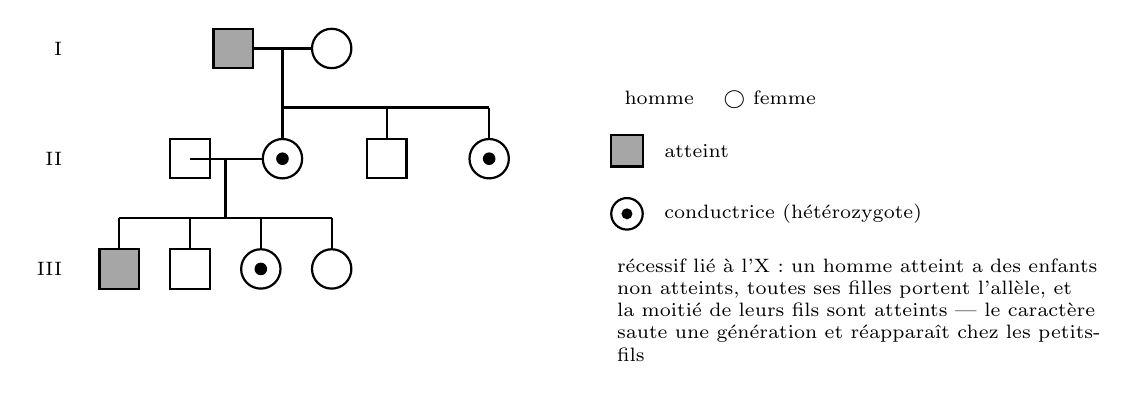
\begin{tikzpicture}[every node/.style={font=\scriptsize}]
  % pedigree: X-linked recessive
  \draw[thick, fill=gray!70] (0,0) rectangle (0.5,0.5); % affected grandfather
  \draw[thick] (1.5,0.25) circle (0.25);
  \draw[thick] (0.5,0.25) -- (1.25,0.25);
  \draw[thick] (0.875,0.25) -- (0.875,-0.5);
  \draw[thick] (0.875,-0.5) -- (3.5,-0.5);
  % children of generation I
  \draw[thick] (0.875,-0.5) -- (0.875,-0.9); \draw[thick, fill=white] (0.875,-1.15) circle (0.25); \fill (0.875,-1.15) circle (0.08);
  \draw[thick] (2.2,-0.5) -- (2.2,-0.9); \draw[thick] (1.95,-1.4) rectangle (2.45,-0.9);
  \draw[thick] (3.5,-0.5) -- (3.5,-0.9); \draw[thick, fill=white] (3.5,-1.15) circle (0.25); \fill (3.5,-1.15) circle (0.08);
  % carrier daughter marries
  \draw[thick] (-0.3,-1.15) -- (0.625,-1.15); \draw[thick] (-0.55,-1.4) rectangle (-0.05,-0.9);
  \draw[thick] (0.15,-1.15) -- (0.15,-1.9); \draw[thick] (-1.2,-1.9) -- (1.5,-1.9);
  \draw[thick] (-1.2,-1.9) -- (-1.2,-2.3); \draw[thick, fill=gray!70] (-1.45,-2.8) rectangle (-0.95,-2.3);
  \draw[thick] (-0.3,-1.9) -- (-0.3,-2.3); \draw[thick] (-0.55,-2.8) rectangle (-0.05,-2.3);
  \draw[thick] (0.6,-1.9) -- (0.6,-2.3); \draw[thick, fill=white] (0.6,-2.55) circle (0.25); \fill (0.6,-2.55) circle (0.08);
  \draw[thick] (1.5,-1.9) -- (1.5,-2.3); \draw[thick, fill=white] (1.5,-2.55) circle (0.25);
  \node[anchor=east] at (-1.8,0.25) {I};
  \node[anchor=east] at (-1.8,-1.15) {II};
  \node[anchor=east] at (-1.8,-2.55) {III};
  % legend
  \node[anchor=west, align=left] at (5,-0.4) {$\square$ homme \quad $\bigcirc$ femme};
  \draw[thick, fill=gray!70] (5.05,-1.25) rectangle (5.45,-0.85); \node[anchor=west] at (5.6,-1.05) {atteint};
  \draw[thick] (5.25,-1.85) circle (0.2); \fill (5.25,-1.85) circle (0.07); \node[anchor=west] at (5.6,-1.85) {conductrice (hétérozygote)};
  \node[anchor=north west, align=left, text width=6.2cm] at (5,-2.3) {récessif lié à l'X~: un homme atteint a des enfants non atteints, toutes ses filles portent l'allèle, et la moitié de leurs fils sont atteints --- le caractère saute une génération et réapparaît chez les petits-fils};
\end{tikzpicture}

{\small \omterm{met:b2:meiosis-heredity:pedigree}{Arbre généalogique} d'un caractère \omterm{def:b2:meiosis-heredity:vocabulary}{récessif} lié à l'X comme
l'hémophilie~: aucune transmission de père à fils, des filles
conductrices, des petits-fils atteints.}
\end{omfigure}

\begin{method}[Lire un arbre généalogique]\label{met:b2:meiosis-heredity:pedigree}
\index{arbre genealogique@arbre généalogique}
\begin{enumerate}
  \item Deux parents non atteints ont un enfant atteint~: le caractère
        est \omterm{def:b2:meiosis-heredity:vocabulary}{récessif} (les deux parents sont \omterm{def:b2:meiosis-heredity:vocabulary}{hétérozygotes}).
  \item Un enfant atteint a toujours un parent atteint, et le caractère
        apparaît à chaque génération~: \omterm{def:b2:meiosis-heredity:vocabulary}{dominant}.
  \item Individus atteints surtout masculins, transmission par des mères
        non atteintes, jamais de père à fils~: \omterm{def:b2:meiosis-heredity:vocabulary}{récessif} lié à l'X.
  \item Un père atteint a toutes ses filles atteintes et aucun fils
        atteint~: \omterm{def:b2:meiosis-heredity:vocabulary}{dominant} lié à l'X.
  \item Transmission par les mères à tous leurs enfants, jamais par les
        pères~: mitochondrial.
  \item Calculer ensuite les probabilités à partir des \omterm{def:b2:meiosis-heredity:vocabulary}{génotypes}
        déduits~: un couple conductrice $\times$ homme sain a une
        probabilité de $\tfrac14$ d'avoir un fils atteint à chaque
        naissance ($\tfrac12$ garçon $\times$ $\tfrac12$
        reçoit l'\omterm{def:b2:meiosis-heredity:vocabulary}{allèle}).
\end{enumerate}
\end{method}

\begin{definition}[L'hérédité extranucléaire]\label{def:b2:meiosis-heredity:extranuclear}
\index{heredite maternelle@hérédité maternelle}\index{heredite mitochondriale@hérédité mitochondriale}
Les mitochondries et les chloroplastes portent leurs propres petits
génomes, en de nombreuses copies par organite et en de nombreux
organites par cellule, et ils proviennent presque entièrement de
l'ovocyte~: le spermatozoïde apporte un noyau et guère plus. Leurs gènes
ont donc une \emph{hérédité maternelle}, sans proportions de
ségrégation~: une mère transmet le caractère à tous ses enfants, un
père à aucun. Les maladies mitochondriales humaines (défauts de la
chaîne respiratoire touchant le muscle et le nerf) suivent ce schéma,
de même que la panachure de certaines plantes, où une cellule mère
contenant à la fois des chloroplastes normaux et mutants les répartit
au hasard entre ses cellules filles, produisant des secteurs verts,
blancs et mixtes. Comme elles ne recombinent jamais, les séquences
mitochondriales retracent les lignées maternelles à travers le temps
--- l'outil du \cref{ch:b2:phylogenetic-trees}.
\end{definition}

\begin{proposition}[L'analyse des tétrades]\label{prop:b2:meiosis-heredity:tetrads}
\index{analyse des tetrades@analyse des tétrades}\index{tetrade ordonnee@tétrade ordonnée}
Chez certains champignons (\emph{Neurospora}, \emph{Sordaria}), les
quatre produits d'une même \omterm{def:b2:meiosis-heredity:meiosis}{méiose} restent ensemble dans un sac,
l'\emph{asque}, et dans l'ordre~: une mitose finale donne huit spores
dont la séquence enregistre les deux divisions. Pour un \omterm{def:b2:meiosis-heredity:vocabulary}{hétérozygote}
$A/a$, un asque de disposition
$4 : 4$ (\emph{ségrégation de première division}) n'a pas connu de
crossing-over entre le gène et son centromère --- les \omterm{def:b2:meiosis-heredity:vocabulary}{allèles} se sont
séparés en anaphase I~; une disposition $2 : 2 : 2 : 2$ ou $2 : 4 : 2$
(\emph{ségrégation de seconde division}) en a connu un, si bien que les
\omterm{def:b2:meiosis-heredity:vocabulary}{allèles} ne se sont séparés qu'en anaphase II. La distance entre le gène
et le centromère vaut la moitié du pourcentage d'asques de seconde
division, car un crossing-over ne recombine que deux des quatre
chromatides. Les tétrades montrent aussi directement que la
recombinaison est réciproque~: toute chromatide recombinée a sa
partenaire complémentaire dans le même asque.
\end{proposition}

\begin{omfigure}
\begin{tikzpicture}[every node/.style={font=\scriptsize}]
  \foreach \dx/\pat/\lab in {0/{omDef,omDef,omDef,omDef,omThm,omThm,omThm,omThm}/{$4:4$, sans\\crossing-over~:\\ségrégation de\\première division}, 4.5/{omDef,omDef,omThm,omThm,omDef,omDef,omThm,omThm}/{$2:2:2:2$,\\crossing-over entre\\gène et centromère}, 9/{omDef,omDef,omThm,omThm,omThm,omThm,omDef,omDef}/{$2:4:2$,\\crossing-over~:\\ségrégation de\\seconde division}} {
    \begin{scope}[xshift=\dx cm]
      \draw[thick, rounded corners=6pt] (0,0) rectangle (0.8,4.2);
      \foreach \c [count=\i] in \pat { \fill[\c] (0.4,4.2-0.5*\i+0.02) circle (0.2); }
      \node[below, align=center] at (0.4,-0.1) {\lab};
    \end{scope}
  }
  \node[anchor=west, align=left, text width=2.6cm] at (12.4,3.2) {asques ordonnés de \emph{Sordaria}~; les spores bleues et rouges portent les deux allèles};
\end{tikzpicture}

{\small \omterm{prop:b2:meiosis-heredity:tetrads}{Tétrades ordonnées}. Sans crossing-over entre le gène et son
centromère, les \omterm{def:b2:meiosis-heredity:vocabulary}{allèles} se séparent à la première division et les huit
spores se lisent $4 : 4$~; avec un crossing-over, ils se séparent à la
seconde division et l'asque se lit $2 : 2 : 2 : 2$ ou $2 : 4 : 2$.}
\end{omfigure}

\section{Exercices}

\begin{exercise}[$\star$]\label{exo:b2:meiosis-heredity:1}
Énumérer quatre différences entre mitose et \omterm{def:b2:meiosis-heredity:meiosis}{méiose} (nombre de
divisions, appariement, produits, identité génétique des produits).
\end{exercise}

\begin{exercise}[$\star$]\label{exo:b2:meiosis-heredity:2}
Combien de gamètes chromosomiquement distincts une personne peut-elle
produire par le seul \omterm{thm:b2:meiosis-heredity:mixing}{brassage interchromosomique}~? Une drosophile ($n = 4$)~? Un pois ($n =
7$)~?
\end{exercise}

\begin{exercise}[$\star$]\label{exo:b2:meiosis-heredity:3}
Chez le pois, le caractère «~tige haute~» ($T$) domine le caractère
«~tige naine~». Donner les proportions phénotypiques et génotypiques de
$Tt \times Tt$ et de $Tt \times tt$. Comment savoir si une plante haute
est $TT$ ou $Tt$~?
\end{exercise}

\begin{exercise}[$\star$]\label{exo:b2:meiosis-heredity:4}
Définir la liaison, la \omterm{def:b2:meiosis-heredity:linkage}{fréquence de recombinaison} et le \omterm{def:b2:meiosis-heredity:linkage}{centimorgan}.
Pourquoi deux gènes situés sur le même chromosome peuvent-ils néanmoins
ségréger comme s'ils étaient indépendants~?
\end{exercise}

\begin{exercise}[$\star\star$]\label{exo:b2:meiosis-heredity:5}
Le \omterm{thm:b2:meiosis-heredity:mendel}{croisement dihybride} de Mendel donna $315$ graines lisses
jaunes, $108$ lisses vertes, $101$ ridées jaunes, $32$ ridées vertes.
Tester l'hypothèse $9 : 3 : 3 :
1$ par un $\chi^2$ (3 degrés de liberté, valeur critique
$7.81$).
\end{exercise}

\begin{exercise}[$\star\star$]\label{exo:b2:meiosis-heredity:6}
Un dihybride $AB/ab$ soumis à un croisement-test donne $412$ $AB$,
$388$ $ab$, $103$
$Ab$, $97$ $aB$. Les gènes sont-ils liés~? Calculer la \omterm{def:b2:meiosis-heredity:linkage}{fréquence de
recombinaison} et la distance génétique~; que donnerait le dihybride $Ab/aB$~?
\end{exercise}

\begin{exercise}[$\star\star$]\label{exo:b2:meiosis-heredity:7}
À l'aide de la fonction de Haldane, convertir $r = 0.20$ et $r = 0.45$
en distances génétiques, et \qty{30}{cM} et \qty{100}{cM} en fractions
de recombinaison. Commenter quelles conversions importent en pratique.
\end{exercise}

\begin{exercise}[$\star\star$]\label{exo:b2:meiosis-heredity:8}
Chez \emph{Drosophila}, l'\omterm{def:b2:meiosis-heredity:vocabulary}{allèle} yeux blancs ($w$) est \omterm{def:b2:meiosis-heredity:vocabulary}{récessif} et lié
à l'X. Donner la descendance, par sexe et par \omterm{def:b2:meiosis-heredity:vocabulary}{phénotype}, de (a) une
femelle blanche $\times$ un mâle rouge, (b) une femelle rouge
\omterm{def:b2:meiosis-heredity:vocabulary}{hétérozygote} $\times$ un mâle blanc, (c) le croisement des filles
de (a) avec leurs frères.
\end{exercise}

\begin{exercise}[$\star\star$]\label{exo:b2:meiosis-heredity:9}
Deux lignées pures de pois de senteur à fleurs blanches, croisées,
donnent une descendance entièrement pourpre qui, autofécondée, donne
$9$ pourpres : $7$ blanches.
Expliquer à l'aide de deux gènes, donner les \omterm{def:b2:meiosis-heredity:vocabulary}{génotypes} des deux lignées
parentales, et prédire le résultat du croisement-test de l'hybride
pourpre.
\end{exercise}

\begin{exercise}[$\star\star\star$]\label{exo:b2:meiosis-heredity:10}
Un croisement-test à trois points donne~: $+++$ 480, $abc$ 470, $+bc$ 11,
$a++$ 9, $++c$ 118, $ab+$ 112, $+b+$ 1, $a+c$ 1 (total 1202). Trouver
l'ordre des gènes, les deux distances, le coefficient de coïncidence et
l'interférence.
\end{exercise}

\begin{exercise}[$\star\star\star$]\label{exo:b2:meiosis-heredity:11}
Chez \emph{Sordaria}, le croisement d'une souche à spores noires avec
une souche à spores beiges donne $700$ asques de disposition $4 : 4$ et
$300$ de dispositions $2 : 2 : 2 : 2$ ou $2 : 4 : 2$. Calculer la
distance entre le gène de la couleur des spores et son centromère, et
expliquer pourquoi le facteur un demi est nécessaire. Schématiser les
chromatides d'une \omterm{def:b2:meiosis-heredity:meiosis}{méiose} qui donne
$2 : 4 : 2$.
\end{exercise}

\begin{exercise}[$\star\star\star$]\label{exo:b2:meiosis-heredity:12}
Le grand-père maternel d'une femme était hémophile~; personne d'autre
n'est atteint dans la famille. Quelle est la probabilité qu'elle soit
conductrice~? Sachant qu'elle a eu deux fils en bonne santé, quelle est
cette probabilité maintenant~? Détailler le raisonnement.
\end{exercise}

\section{Problème~: croisements dans la salle des mouches}

\begin{problem}[{Problème du week-end --- des croisements de
\emph{Drosophila} analysés depuis la proportion de monohybridisme
jusqu'à une carte à trois points, et un \omterm{met:b2:meiosis-heredity:pedigree}{arbre généalogique} humain
calculé, jusqu'à la carte de trois gènes liés à l'X et à leur
interférence}]
\label{pb:b2:meiosis-heredity:1}
Les caractères ailes vestigiales ($vg$) et corps ébène ($e$) sont
\omterm{def:b2:meiosis-heredity:vocabulary}{récessifs} et portés par des autosomes différents~; corps noir ($b$) et
$vg$ sont \omterm{def:b2:meiosis-heredity:vocabulary}{récessifs} et tous deux portés par le chromosome 2~; corps
jaune ($y$), yeux blancs ($w$) et ailes miniatures
($m$) sont \omterm{def:b2:meiosis-heredity:vocabulary}{récessifs} et liés à l'X. Valeurs critiques du $\chi^2$ à
\qty{5}{\%}~: $3.84$ (1 d.d.l.), $7.81$ (3 d.d.l.).

\medskip
\noindent\textbf{Partie I --- Deux gènes autosomiques.}
Une mouche vestigiale pure est croisée avec une mouche ébène pure~; les
$F_1$ sont toutes de type sauvage~; on examine $1600$ mouches $F_2$~:
$892$ sauvages, $309$
vestigiales, $296$ ébène, $103$ vestigiales ébène.
\begin{enumerate}
  \item Donner les \omterm{def:b2:meiosis-heredity:vocabulary}{génotypes} des parents, des $F_1$ et des gamètes
        des $F_1$.
  \item Calculer les effectifs attendus sous l'hypothèse d'un brassage
        indépendant.
  \item Calculer le $\chi^2$ et conclure.
  \item Quelle fraction des mouches $F_2$ de type sauvage est \omterm{def:b2:meiosis-heredity:vocabulary}{homozygote}
        aux deux loci~?
  \item La $F_1$ est croisée avec une mouche vestigiale ébène~: prédire
        les quatre classes et leurs proportions.
  \item Des mouches ébène élevées à \qty{29}{\celsius} sont plus pâles
        qu'à \qty{18}{\celsius}. Qu'est-ce que cela indique sur la
        relation entre \omterm{def:b2:meiosis-heredity:vocabulary}{génotype} et \omterm{def:b2:meiosis-heredity:vocabulary}{phénotype}~?
\end{enumerate}

\medskip
\noindent\textbf{Partie II --- Deux gènes liés.}
Une mouche noire pure est croisée avec une mouche vestigiale pure~; les
femelles $F_1$ sont croisées avec des mâles noirs vestigiaux~: $965$
noires,
$944$ vestigiales, $206$ noires vestigiales, $185$ de type sauvage.
\begin{enumerate}[resume]
  \item Écrire le \omterm{def:b2:meiosis-heredity:vocabulary}{génotype} de la $F_1$, en montrant quels \omterm{def:b2:meiosis-heredity:vocabulary}{allèles} sont
        sur le même chromosome.
  \item Identifier les classes parentales et recombinées, et expliquer
        pourquoi le type sauvage est ici un \emph{recombiné}.
  \item Calculer $r$ et la distance génétique.
  \item La corriger à l'aide de la fonction de Haldane.
  \item Le même croisement-test réalisé avec des \emph{mâles} $F_1$ ne
        donne que deux classes, noire et vestigiale, en nombres égaux.
        Que montre ce résultat sur la \omterm{def:b2:meiosis-heredity:meiosis}{méiose} des mâles de drosophile~?
  \item Prédire les classes et leurs proportions si la femelle $F_1$
        était issue d'un croisement noir vestigial $\times$ sauvage.
\end{enumerate}

\medskip
\noindent\textbf{Partie III --- Un \omterm{met:b2:meiosis-heredity:pedigree}{arbre généalogique} humain.}
L'hémophilie A est récessive et liée à l'X. Un homme hémophile a une
fille, qui épouse un homme non atteint.
\begin{enumerate}[resume]
  \item Quel est le \omterm{def:b2:meiosis-heredity:vocabulary}{génotype} de la fille, et pourquoi est-il certain~?
  \item Probabilité que son premier enfant soit un fils atteint.
  \item Probabilité qu'une de ses filles soit conductrice.
  \item Probabilité que, parmi ses trois enfants, aucun ne soit
        atteint.
  \item Expliquer pourquoi la maladie n'est jamais transmise de père à
        fils, et comment une femme pourrait être atteinte.
  \item La sœur de l'homme atteint a deux fils en bonne santé~; leur
        mère (la mère de l'homme) était conductrice. Calculer la
        probabilité que la sœur soit conductrice, avant et après avoir
        pris ses fils en compte.
\end{enumerate}

\medskip
\noindent\textbf{Partie IV --- Trois gènes liés à l'X.}
Une femelle $y\,w\,m/+\,+\,+$ est croisée avec un mâle $y\,w\,m$~; on
examine ses $2000$
fils~: $+++$ 853, $ywm$ 833, $y++$ 24, $+wm$ 26, $yw+$ 128,
$++m$ 132, $+w+$ 2, $y+m$ 2.
\begin{enumerate}[resume]
  \item Pourquoi peut-on examiner directement les fils, sans
        croisement-test~?
  \item Identifier les classes parentales et doubles crossing-over, et
        en déduire l'ordre des gènes.
  \item Calculer les deux \omterm{def:b2:meiosis-heredity:linkage}{fréquences de recombinaison} et tracer la
        carte.
  \item Calculer le nombre attendu de doubles crossing-over, le
        coefficient de coïncidence et l'interférence.
  \item Calculer directement à partir des données la \omterm{def:b2:meiosis-heredity:linkage}{fréquence de
        recombinaison} entre les deux gènes extrêmes, et expliquer
        pourquoi elle est inférieure à la somme des deux distances.
  \item À quoi ressembleraient les filles de ce croisement, et pourquoi
        sont-elles inutilisables pour la cartographie~?
  \item Énoncer le résultat~: la carte des trois gènes et
        l'interférence.
\end{enumerate}
\end{problem}
